\documentclass{beamer}

\usepackage[utf8]{inputenc}
\usepackage{fancybox,fancyvrb}
\usepackage{environ}
\usepackage{tikz}

\beamertemplatenavigationsymbolsempty
\setbeamertemplate{footline}[frame number]
\usetheme{Pittsburgh}

\newcommand{\grad}{\nabla}
\newcommand{\ih}{\boldsymbol{\hat{\textbf{\i}}}}
\newcommand{\jh}{\boldsymbol{\hat{\textbf{\j}}}}
\newcommand{\vF}{\boldsymbol{\vec{\textbf{F}}}}

\title{2.4 A Numerical Method (Euler's Method)}

\subtitle{a lesson for MATH F302 Differential Equations}

\author{Ed Bueler, Dept.~of Mathematics and Statistics, UAF}

\date{\tiny \today}


\begin{document}
\setbeamertemplate{itemize item}{$\bullet$}
\setbeamertemplate{itemize subitem}{$\circ$}

\begin{frame}
\titlepage

\centerline{\tiny for textbook: \, D. Zill, \emph{A First Course in Differential Equations with Modeling Applications}, 11th ed.}
%\color{green!40!blue}
\end{frame}



\begin{frame}{where we stand}

\begin{itemize}
\item we have methods from recent sections for generating by-hand solutions to first-order differential equations:
    \begin{itemize}
    \item[2.2] separable equations: $y'=g(x)h(y)$
    \item[2.3] linear equations: $y'+P(x)y=f(x)$
    \item[2.4] exact equations: $M\,dx + N\,dy=0$ where $\frac{\partial M}{\partial y} = \frac{\partial N}{\partial x}$
    \end{itemize}
\item there are further methods \dots such as in section 2.5
    \begin{itemize}
    \item but \alert{we are skipping \S 2.5} because these methods are un-memorable and weak IMHO
    \end{itemize}

\bigskip
\item where do we stand?:
\begin{quote}
there are some problems we can do, but many for where our by-hand calculus/algebra techniques so far \alert{don't} work
\end{quote}
\end{itemize}
\end{frame}


\begin{frame}{example 1}

\begin{itemize}
\item Example 1.  solve the initial value problem
    $$\frac{dy}{dt} = t-y^2, \qquad y(0)=1$$
in particular, find $y(4)$
\end{itemize}

\medskip
Solution version 0: \emph{Explain why the previous methods don't apply.}

\vspace{50mm}
\end{frame}


\begin{frame}{example 1, cont.}

Solution version 1: \emph{Solve it using a direction field and a pen.}

\bigskip
\hfill 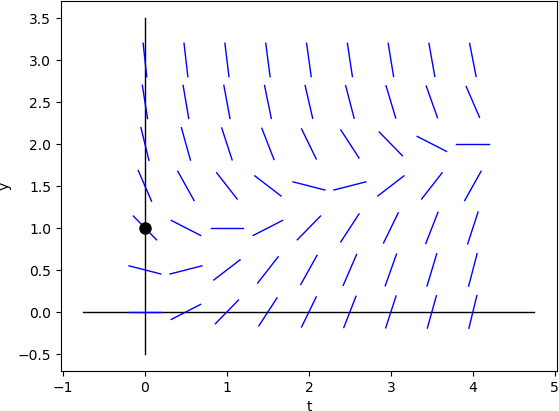
\includegraphics[width=0.7\textwidth]{figs/sequence-1}

\begin{itemize}
\item this is only approximate
\end{itemize}
\end{frame}


\begin{frame}{example 1, cont.~cont.}

Solution version 2: \emph{Make a computer follow the direction field.}

\bigskip
\hfill 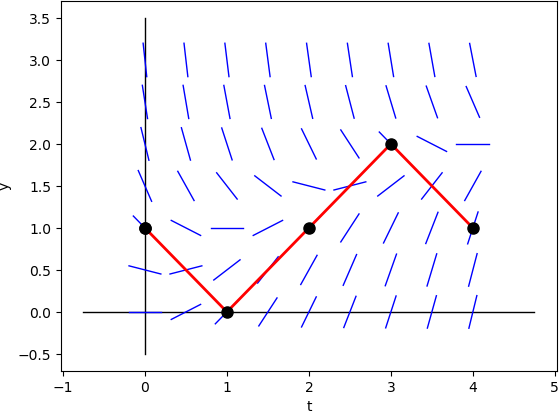
\includegraphics[width=0.7\textwidth]{figs/sequence-2}

\begin{itemize}
\item this is still only approximate because we go straight
\end{itemize}
\end{frame}


\begin{frame}{example 1, cont.~cont.~cont.}

Solution version 3: \emph{The direction field is not actually needed.}

\bigskip
\hfill 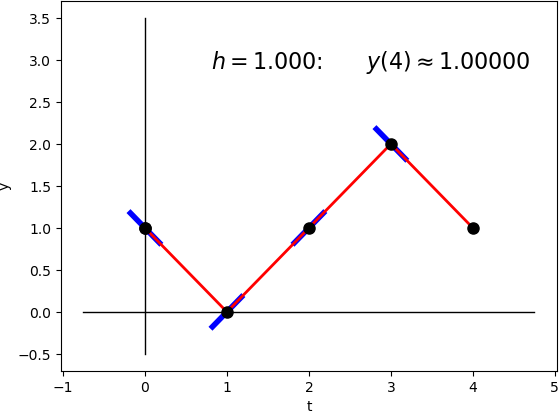
\includegraphics[width=0.7\textwidth]{figs/sequence-3}

\begin{itemize}
\item this is the same as previous
\end{itemize}
\end{frame}


\begin{frame}{example 1, cont.~cont.~cont.~cont.}

Solution version 4: \emph{Do it more accurately by smaller steps}

\bigskip
\hfill 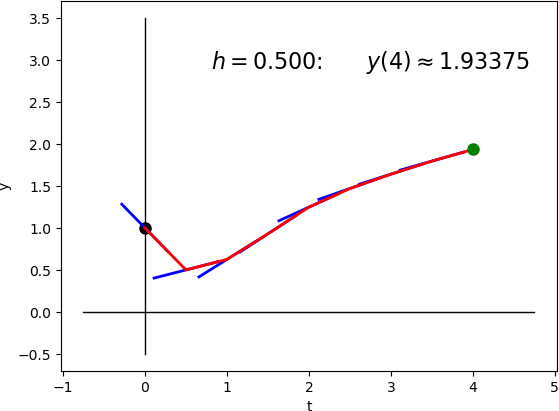
\includegraphics[width=0.7\textwidth]{figs/sequence-4}

\begin{itemize}
\item the blue slope lines are not really needed \dots
\end{itemize}
\end{frame}


\begin{frame}{example 1, cont.$^5$}

Solution version 5: \emph{Smaller steps.}

\bigskip
\hfill 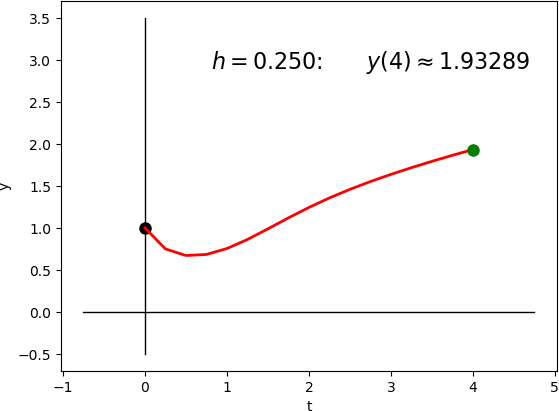
\includegraphics[width=0.7\textwidth]{figs/sequence-5}

\begin{itemize}
\item this is \emph{still} only approximate
\end{itemize}
\end{frame}


\begin{frame}{example 1, cont.$^6$}

Solution version 6: \emph{Smaller.  (Make the computer do more work.)}

\bigskip
\hfill 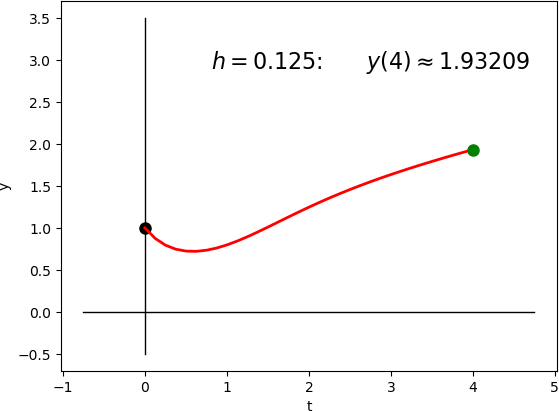
\includegraphics[width=0.7\textwidth]{figs/sequence-6}

\begin{itemize}
\item this looks like a \emph{solution} not a direction field 
\end{itemize}
\end{frame}


\begin{frame}{Euler's method}

\begin{itemize}
\item the idea of following the direction field, in a straight line for a short distance, and repeating, is \emph{Euler's method}
\item for the differential equation $\frac{dy}{dx} = f(x,y)$, Euler's method is
        $$y_{n+1} = y_n + h\, f(x_n,y_n)$$

\vspace{-2mm}
    \begin{itemize}
    \item $h\ne 0$ is a step size you get to choose
    \item the next $x$-value is always $h$ away from the last: $x_{n+1} = x_n + h$
    \item this is a formula to understand \emph{and} memorize
    \item \dots and to put in computer programs
    \end{itemize}
\item in the previous slides we had $f(x,y)=x-y^2$, starting values $(x_0,y_0)=(0,1)$, and four values of $h$: $h=1,0.5,0.25,0.125$
\end{itemize}
\end{frame}


\begin{frame}{a derivation of Euler's method}

\begin{itemize}
\item easy to derive it from the direction field of $\frac{dy}{dx} = f(x,y)$
\item suppose we are at a point $(x_n,y_n)$
    \begin{itemize}
    \item this might be the initial point $(x_0,y_0)$
    \end{itemize}
\item the slope is $m=f(x_n,y_n)$ so the line we want is
    $$y-y_n = f(x_n,y_n)(x-x_n)$$
\item we want to move to a new location $x_{n+1}=x_n+h$ so $x-x_n=h$ and $y=y_{n+1}$
\item thus
    $$y_{n+1} = y_n + h\, f(x_n,y_n)$$
\end{itemize}
\end{frame}


\begin{frame}{example 2}

\begin{itemize}
\item X
\end{itemize}
\end{frame}


\begin{frame}{X}

\begin{itemize}
\item X
\end{itemize}
\end{frame}


\begin{frame}{X}

\begin{itemize}
\item X
\end{itemize}
\end{frame}


\begin{frame}[fragile]
\frametitle{example 5, finished}

\begin{itemize}
\item[(c)] contour plot \dots here is Matlab/Octave code:
\begin{Verbatim}[fontsize=\footnotesize]
f = @(x,y) y.*(1.0 - 1.0./(x.^2+y.^2));    % define function
x = -3:.1:3;  [xx,yy] = meshgrid(x,x);     % grid of points
c = -0.8:0.2:0.8;                          % contours we want
h = contour(xx,yy,f(xx,yy),c,'k');         % black contours
clabel(h)                                  % ... with labels
axis equal                                 % looks better
\end{Verbatim}
\end{itemize}
\end{frame}


\begin{frame}{expectations}

\begin{itemize}
\item to learn this material, just watching this video is \emph{not} enough!

\item also:
     \begin{itemize}
     \item \emph{watch} ``found online'' videos at

     \centerline{\href{https://bueler.github.io/math302/week4.html}{\tt \color{cyan} bueler.github.io/math302/week4.html}}
     \item \emph{try-out} Euler's method codes at the same link
     \item \emph{read} section 2.6 in the textbook
     \item \emph{do} the WebAssign exercises for section 2.6
     \end{itemize}
\end{itemize}
\end{frame}

\end{document}

